\chapter{Description du dataset (MOUS)}

On va dans cette partie présenter le jeu de données MEG sur lequel j'ai travaillé et expliciter les différents stimuli de compréhension linguistique auxquels les sujets ont été soumis. Cela nous permettra de nous approprier les données et de bien comprendre le protocole expérimental auquel les sujets ont été soummis. 
On souhaite appliquer notre algorithme à un dataset public d'étude de la compréhension linguistique, le Mother Of Unification Studies (MOUS) \cite{4}. 

L'étude a été réalisée sur un total 204 locuteurs natifs de Hollande et ayant comme langue maternelle le néerlandais. Il y a 100 hommes et 104 femmes, d'un âge moyen de 22 ans (de 18 à 33 ans). Dans la procédure de consentement éclairé, les sujets ont explicitement consenti à ce que les données anonymes collectées soient utilisées à des fins de recherche. Chaque sujet a effectué soit la tâche visuelle, soit celle auditive. Tous les sujets étaient droitiers, avaient une vision normale ou corrigée par le port de lunettes de vue. Ils n'avaient pas d'antécédents de déficits neurologiques, développementaux ou linguistiques. 

\vspace{2mm}
Ce dataset est structuré de la façon suivante : 
Il y a un total de 204 sujets répartis en deux moitiés pour deux tâches de compréhension linguistique différentes, une tâche visuelle et une tâche auditive. Pour chaque sujet, on dispose d'un enregistrement MEG d'une durée d'environ 1 heure.

\begin{figure}[!ht]
    \centering
    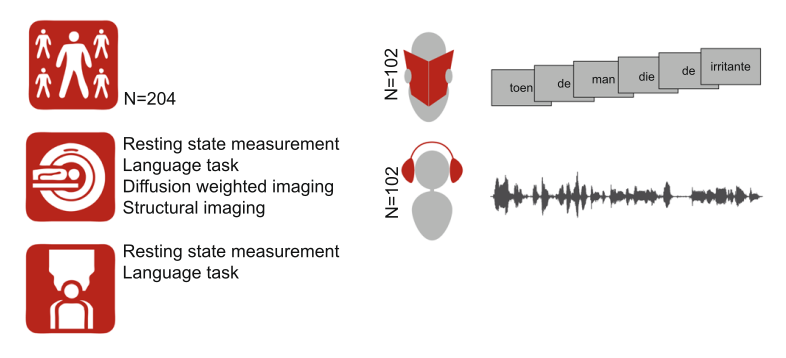
\includegraphics[width=10cm]{orga_dataset.png}
    \caption{Organisation du dataset. Issu de \cite{4}}
    \label{fig2.1}
\end{figure}

Les stimuli sont composés de 360 phrases en hollandais et leur analogues mélangés i.e une phrase ayant subi des permutations aléatoires entre les différents mots (donc inintelligibles a priori).

On a alors 
\begin{enumerate}
    \item 360 phrases, simples ou complexes (grammaticalement parlant)
    \item 360 listes aléatoires de mots 
\end{enumerate}

On rappelle qu'une phrase simple ne comporte qu'une seule proposition, donc un verbe conjugué. Tandis qu'une phrase complexe comporte plusieurs propositions, donc plusieurs verbes conjugués. Il y a donc naturellement plus de COD, COI et subordonnées au sein d'une phrase complexe.

\vspace{2ex}
Les phrases sont composées de 9 à 15 mots. Parmi ces différentes phrases, il y a :
\begin{enumerate}
    \item 180 phrases simples appelées simple relative clause sentence (RC-)
    \item 180 phrases complexes appelées relative clause sentence (RC+)
\end{enumerate}

\begin{figure}[!ht]
    \centering
    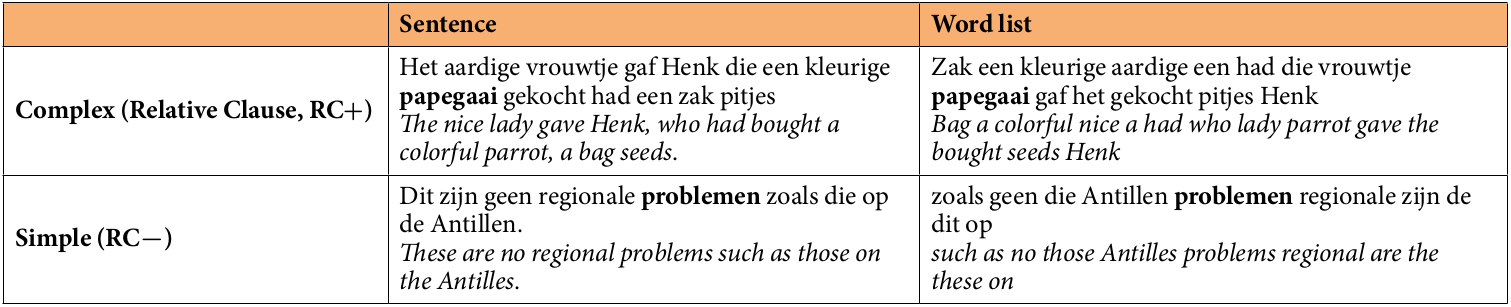
\includegraphics[width=20cm]{stimuli.png}
    \caption{Exemple des différents stimuli : Phrase simple (RC- sentence), phrase complexe (RC+ sentence) et listes aléatoires de mots associées. Issu de \cite{4}}
    \label{fig2.2}
\end{figure}

Chaque sujet est soumis à 180 phrases simples ou complexes donc à 180 sentences (RC+ ou RC-) ainsi qu’à 180 liste de mots aléatoires ou Random lists.

\vspace{2ex}
Sur chaque sujet, les phrases et les listes de mots aléatoires ont été utilisé le même nombre de fois.
Chaque phrase et sa liste de mots aléatoire associée contiennent un nom commun qui se trouve à la même position. Cette position peut varier de la 3ième à la 13ième position et ce mot est annoté comme cible ("target word").
Le mot placé en amont du "target word" ne diffère en taille d'un maximum de deux lettres entre la phrase et la liste de mots aléatoire associée.

\vspace{2ex}
Les stimuli sont soumis par blocs de 5 phrases ou 5 listes aléatoires de mots. Au début de chaque bloc, une présentation de 1500 ms indiquait le type de bloc : zinnen (phrases) ou woorden (mots). Dans les phrases, le premier mot commençait par une majuscule et le dernier mot se terminait par un point. 

\vspace{2ex}L'intervalle entre les essais a été réparti entre 3200 et 4200 ms. Pendant cette période, un écran vide était présenté, suivi d'une croix de fixation. C'est la phase d'instructions identifiée comme "Fixation picture, pre-trial baseline" et indexée par le nombre 20.

\begin{figure}[!ht]
    \centering
    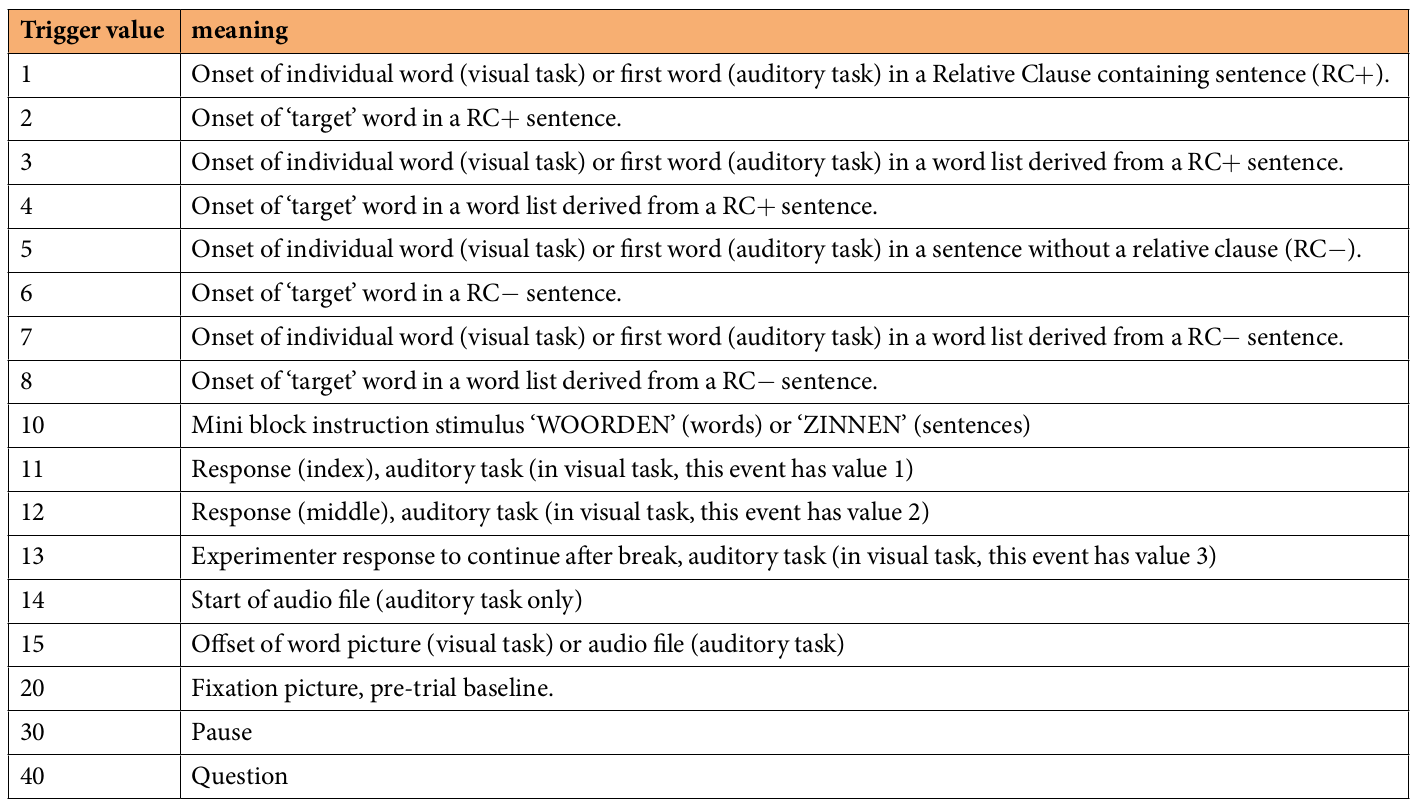
\includegraphics[width=20cm]{events_id.png}
    \caption{Identification des différents évènements et stimuli lors de l'enregistrement de la tâche de compréhension. Issu de \cite{4}}
    \label{fig2.3}
\end{figure}

Ce document va nous permettre d'identifier quels stimuli sont envoyés, un à un. Lors de l'analyse, cela permettra de segmenter les séries temporelles en courtes séquences appelées "époques" et donc de se focaliser sur les activités cérébrales d'intérêt par rapport à la tâche de compréhension linguistique.

\vspace{2ex}
On verra dans la partie suivante le pré-traitement que j'ai effectué sur les données ainsi que la manière dont j'ai segmenté le signal sur la base des différentes conditions expérimentales en se basant sur les événements.
